\documentclass[compress]{beamer}

\usepackage{xmpmulti}

\usepackage{graphicx,float}
\usepackage{amsfonts}
\usepackage{mdwlist}
\usepackage{colortbl}

\pgfdeclareimage[width=\paperwidth]{mybackground}{../../common/boulder.pdf}


\newcommand{\danquote}[1]{

\begin{flushright}
\begin{overpic}[width=5.5cm,tics=10]{general_figures/speech_bubble}
	\put(10,30) { \parbox{4cm}{#1 }}
\end{overpic}

\includegraphics[width=1.5cm]{general_figures/milkman_dan}
\end{flushright}
}

\newcommand{\explain}[2]{\underbrace{#2}_{\mbox{\footnotesize{#1}}}}
\newcommand{\e}[2]{\mathbb{E}_{#1}\left[ #2 \right] }
\newcommand{\ind}[1]{\mathbb{I}\left[ #1 \right] }
\newcommand{\ex}[1]{\mbox{exp}\left\{ #1\right\} }
%\newcommand{\g}{\, | \,}
\newcommand{\citename}[1]{#1 }

\newcommand{\greentext}[1]{\textcolor{caribbeangreen}{#1}}
\newcommand{\yellowtext}[1]{\textcolor{amber}{#1}}
\newcommand{\redtext}[1]{\textcolor{red}{#1}}
\newcommand{\bluetext}[1]{\textcolor{blue}{#1}}

\newcommand{\bm}[1]{\mbox{\boldmath$#1$}}
\newcommand{\Dir}{\mathrm{Dir}}
\newcommand{\Mult}{\mathrm{Mult}}
\newcommand{\g}[1]{\Gamma \left( #1 \right)}
\newcommand{\paragraph}[1]{ \vskip 1cm {\bf \large #1}}

\newcommand{\tb}[1]{\textbf{#1}}
\newcommand{\subtwo}[2]{_{#1, #2}}
\newcommand{\subthree}[3]{_{#1, #2, #3}}
\newcommand{\minussubtwo}[2]{_{-{#1, #2}}}
\newcommand{\minussubthree}[3]{_{-{#1, #2, #3}}}
\newcommand{\suptwo}[2]{^{#1, #2}}
\newcommand{\supthree}[3]{^{#1, #2, #3}}
\newcommand{\minussuptwo}[2]{^{-{#1, #2}}}
\newcommand{\minussupthree}[3]{^{-{#1, #2, #3}}}
\newcommand{\prior}[1]{\mathcal{B}#1} % to be revised

\newcommand{\gfx}[2]{
\begin{center}
	\includegraphics[width=#2\linewidth]{teaparty/figures/#1}
\end{center}
}


\usetheme[bullet=circle,                     % Use circles instead of squares for bullets.
          titleline=true,                    % Show a line below the frame title.
          showdate=true,                     % show the date on the title page
          alternativetitlepage=true,         % Use the fancy title page.
          titlepagelogo=general_figures/culogo,              % Logo for the first page.
          % Logo for the header on first page.
          headerlogo=general_figures/boulder_cs,
          ]{UCBoulder}

\usecolortheme{ucdblack}
\title[ITM]{Creating and Evaluating Multilingual Topic Models}
\author[Boyd-Graber]{Shudong Hao~(UCB), Mans Hulden~(UCB), Jordan Boyd-Graber~(UCB), Philip~Resnik~(UMD)}
\date{December 2015}

\institute[Boulder] % (optional, but mostly needed)
{University of Maryland and University of Colorado Boulder}

%\AtBeginSection[] % "Beamer, do the following at the start of every section"
%{ \begin{frame} \frametitle{Outline} % make a frame titled "Outline"
%\tableofcontents[currentsection] % show TOC and highlight current section
%\end{frame} }

\begin{document}


\maketitle


\begin{frame}{Goal: Consistent Representations Across Languages}
  \begin{itemize}
    \item Learn multilingual topics that can serve as
      bridges between languages
    \item Goal 1: Aid understanding of analyst (multilingual or
      monolingual)
    \item Goal 2: Serve as machine representation for classification
      into ontology
  \end{itemize}

  \begin{center}
    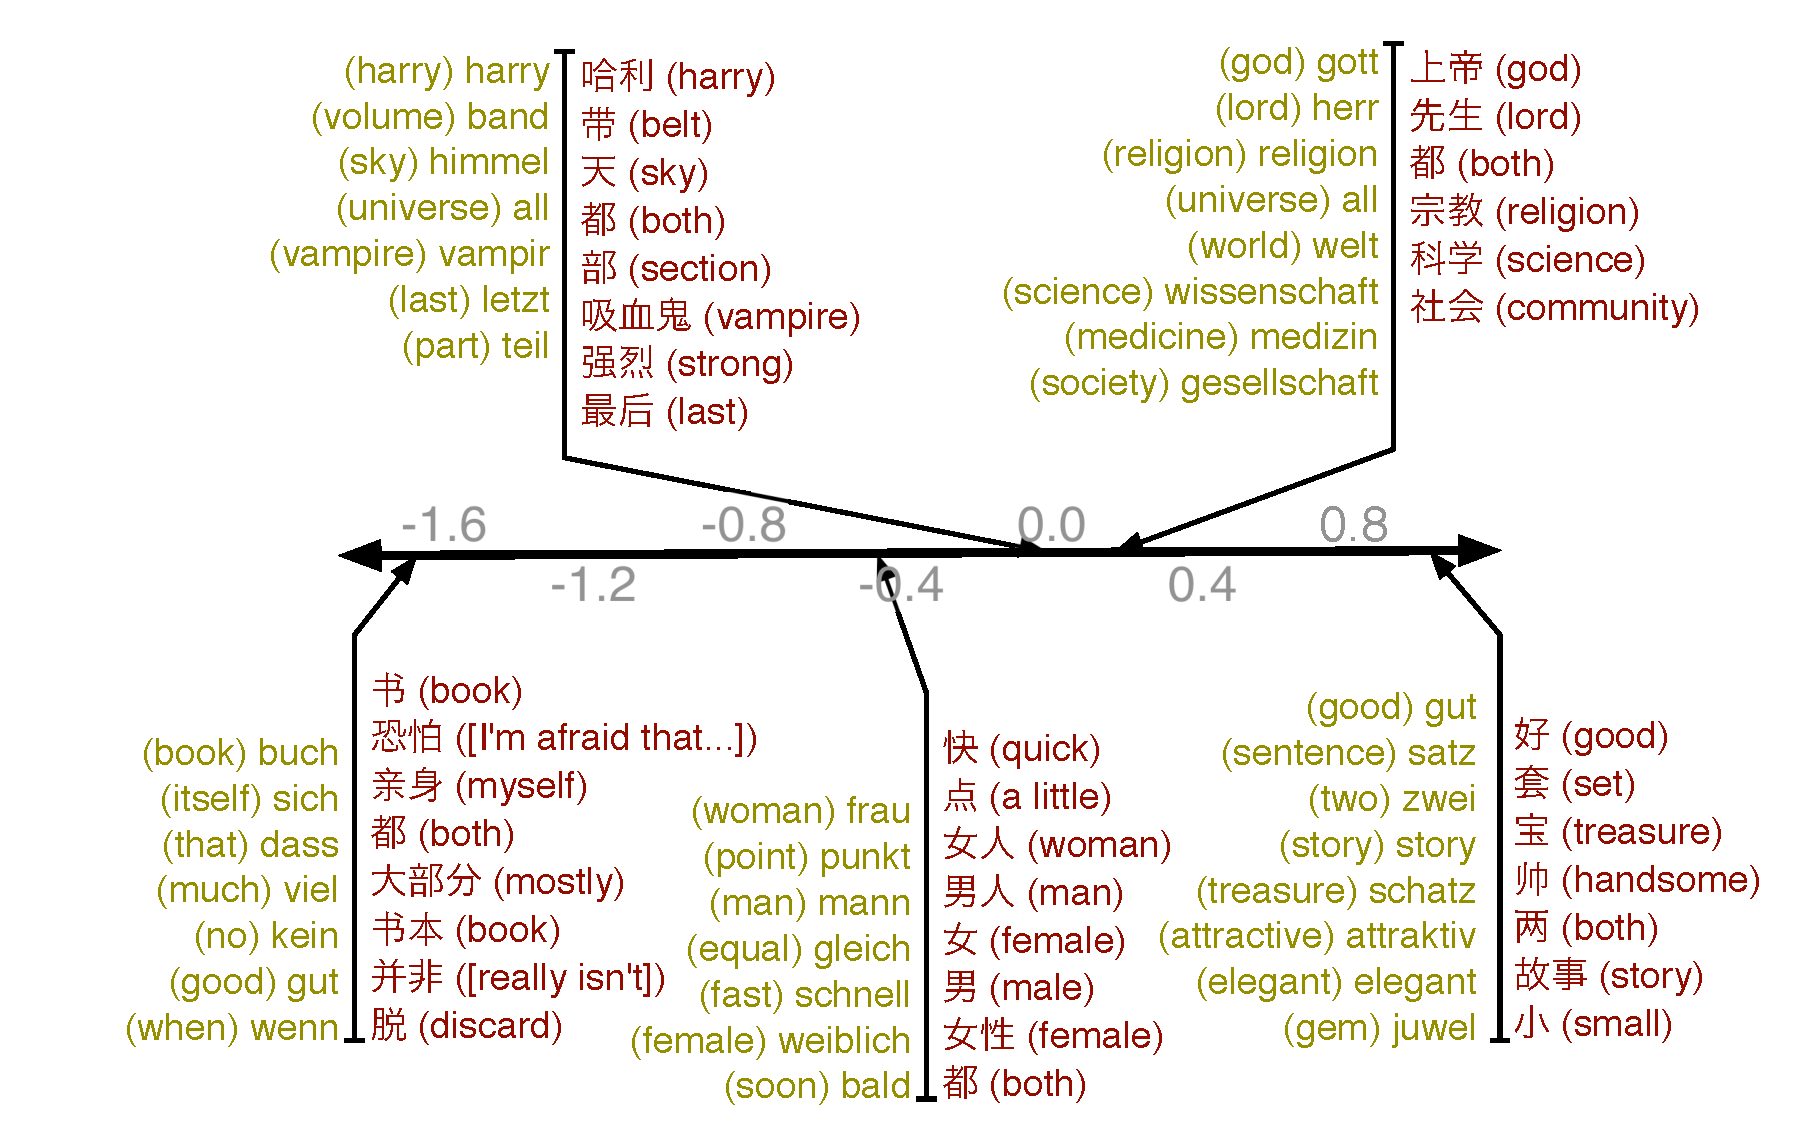
\includegraphics[width=.6\linewidth]{mlslda/chinese_amazon_dict}
  \end{center}

\end{frame}

	\begin{frame}{Document-Links Model}
		\begin{center}
			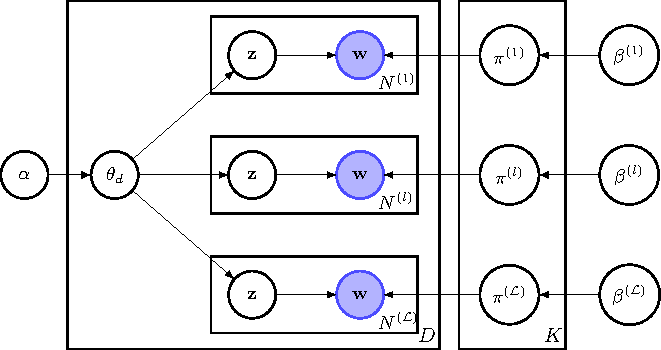
\includegraphics[height=0.4\textheight]{multilingual_itm/polylingual-new.pdf}
		\end{center}
		\begin{itemize}
			\item Use documents about the same subject to
                          create links across languages (e.g., these
                          documents discuss the same election in
                          Arabic and English)
		\end{itemize}
	\end{frame}
	\begin{frame}{Vocabulary-Links Model}
		\begin{center}
			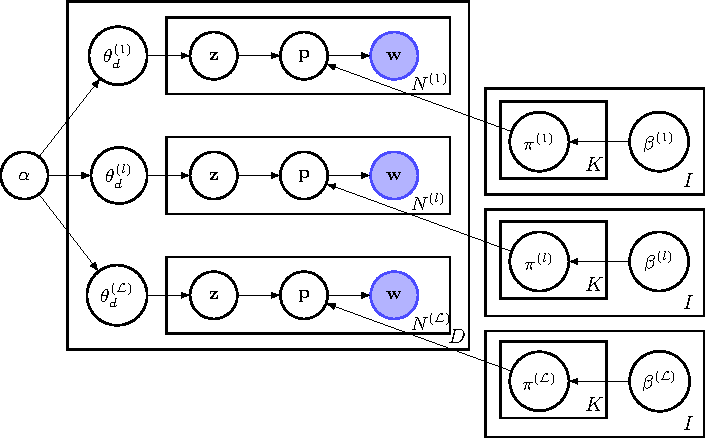
\includegraphics[height=0.4\textheight]{multilingual_itm/treeprior.pdf}
		\end{center}
		\begin{itemize}
		\item Use dictionary (i.e., Wiktionary) as the
                  dictionary to create links between words (i.e., if
                  ``fromage'' is in a topic in French, ``cheese''
                  should be in English)
	\end{itemize}
	\end{frame}
	\begin{frame}{Combined Model}
		\begin{center}
			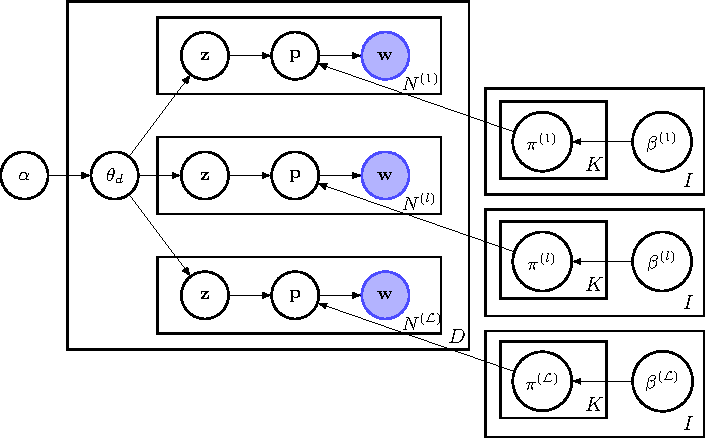
\includegraphics[height=0.4\textheight]{multilingual_itm/link-prior.pdf}
		\end{center}
		\begin{itemize}
			\item Allow for either information about
                          documents or words to improve multilingual topics
		\end{itemize}
	\end{frame}


\begin{frame}{Problem: Detecting Good Multilingual Topics}

\begin{itemize}
  \item If we don't understand the language, how do we know if we have
    good topics?
  \item Need metrics that:
  \begin{itemize}
    \item Are simple, not dependent on expensive resources
    \item Correlate well with classification accuracy
    \item Relatively language independent
   \end{itemize}
\pause
\item NPMI and human judgements
\end{itemize}
\end{frame}

	\begin{frame}{TED Talk Translations}
	    \begin{itemize}
	      \item Languages: English, Chinese, Turkish;
	      \item $970$ documents in each language;
	      \item Labeled with topics (business, society, technology)
	    \end{itemize}
	\end{frame}



	\begin{frame}{Wikipedia}
		\begin{itemize}
			\item Obtained from \url{http://linguatools.org/tools/corpora/wikipedia-comparable-corpora/};
			\item Languages: English, Chinese, Turkish;
			\item $62,352$ documents in each language;
			\item Used for evaluating NPMI scores.
		\end{itemize}
	\end{frame}

	\begin{frame}{Brief News}
		\begin{itemize}
			\item Provided by LORELEI;
			\item Languages: English, Uzbek;
			\item $1,731$ documents in each language;
			\item Working on hand-annotation of topic (not complete)
		\end{itemize}
	\end{frame}
	

		\begin{frame}{Normalized Mutual Pointwise Information (NPMI)}
			\begin{itemize}
				\item \textbf{NPMI-Internal} focuses on a single language;
					\begin{align}
					NPMI(w_i,w_j)=\frac{\log\left(\frac{\Pr(w_i,w_j)}{\Pr(w_i)\Pr(w_j)}\right)}{-\log\Pr(w_i,w_j)}.
					\end{align}
			\item Correlates well with human judgements of
                          topic quality
			\end{itemize}
			\begin{center}
				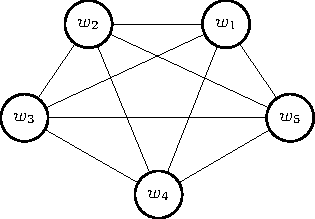
\includegraphics[height=0.3\textheight]{multilingual_itm/npmi-internal.pdf}
			\end{center}
		\end{frame}


		\begin{frame}{Normalized Mutual Pointwise Information (NPMI)}
			\begin{itemize}
				\item \textbf{NPMI-Cross} focuses on language pairs;
				\begin{align}
				NPMI\left(w_i^{(l_1)},w_j^{(l_2)}\right)=\frac{\log\left(\frac{\Pr(w_i,w_j)}{\Pr(w_i)\Pr(w_j)}\right)}{-\log\Pr(w_i,w_j)}.
				\end{align}
			\begin{center}
				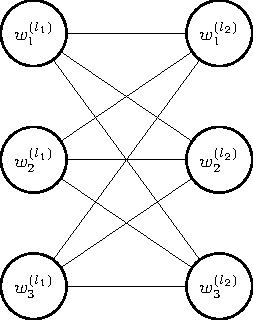
\includegraphics[height=0.3\textheight]{multilingual_itm/npmi-cross.pdf}
			\end{center}

				\item When there are more than two languages, we calculate the NPMI-Cross for each pair of languages and take the average.			
				\item Seems to work well even with
                                  very limited parallel data
			\end{itemize}
		\end{frame}
		

		\begin{frame}{Classification}

                  \begin{columns}
                    \column{.3\linewidth}
			\begin{itemize}
				\item Topic distribution of $l_1$ docs
                                  train SVM
				\item Test on topic distribution of $l_2$ docs
				\item Classification correlates
                                  well with cross-NPMI.
			\end{itemize}
                    \column{.6\linewidth}
                    \only<1>{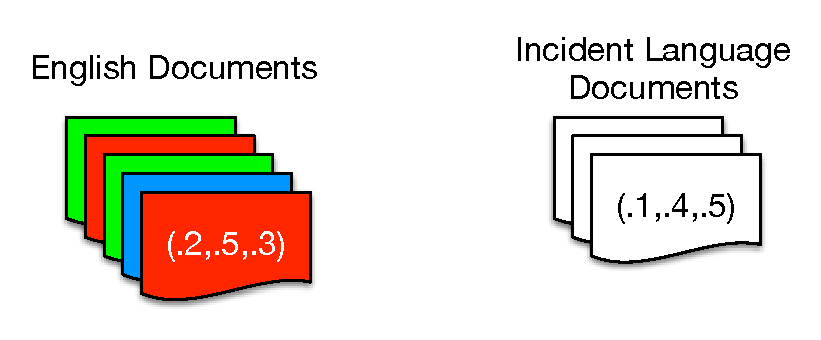
\includegraphics[width=1.0\linewidth]{multilingual_itm/classification_1}}
                    \only<2>{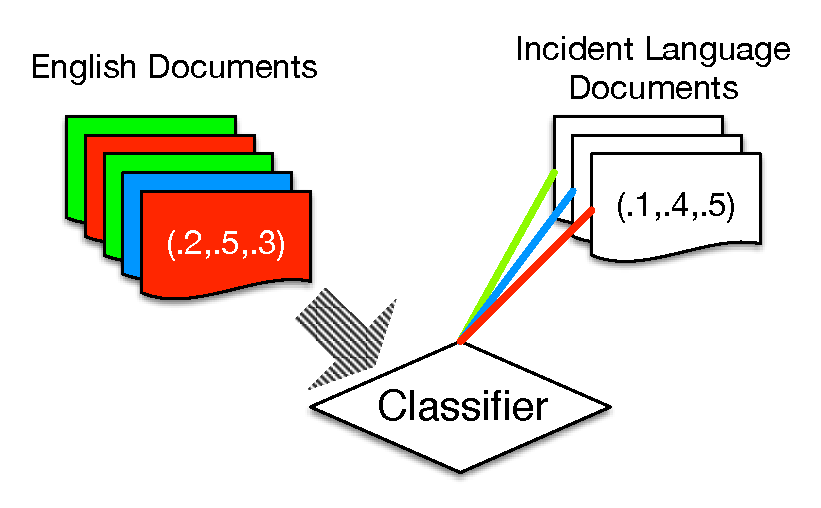
\includegraphics[width=1.0\linewidth]{multilingual_itm/classification_2}}
                    \end{columns}
		\end{frame}
	


	
	% \begin{frame}{Dataset}
	% 	Note on the corpus:
	% 	\begin{itemize}
	% 		\item It requires multilingual labeled corpus;
	% 		\item I still use TED Talks 2013, since each article has many categories that can be used as labels;
	% 		\item I choose \textbf{art} and \textbf{biology} as labels, since there are only three articles contain both labels. They have the minimal overlaps and comparable amounts of documents in each label;
	% 		\item \textbf{Art}: $122$ documents in each language;
	% 		\item \textbf{Biology}: $88$ documents in each language.
	% 	\end{itemize}
	% \end{frame}

	
	\begin{frame}{English and Chinese}
		\begin{itemize}
			\item Correlation between \textbf{classification accuracy} and \textbf{NPMI-Internal}:
			\begin{itemize}
				\item English: $0.8309$
				\item Chinese: $0.8095$
			\end{itemize}
			\item Correlation between \textbf{average classification accuracy} and \textbf{NPMI-Cross}:
			\begin{itemize}
				\item $0.8216$
			\end{itemize}			
		\end{itemize}
		\begin{center}
			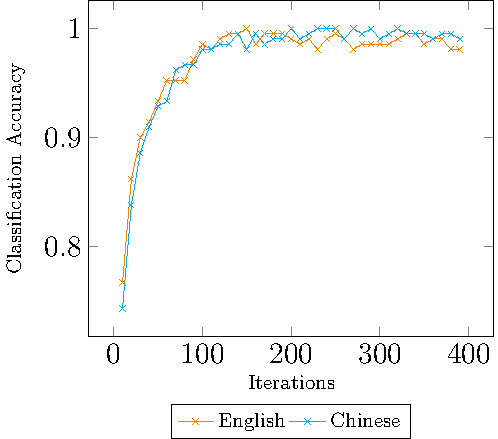
\includegraphics[height=0.5\textheight]{multilingual_itm/clf-en-cmn.pdf}
			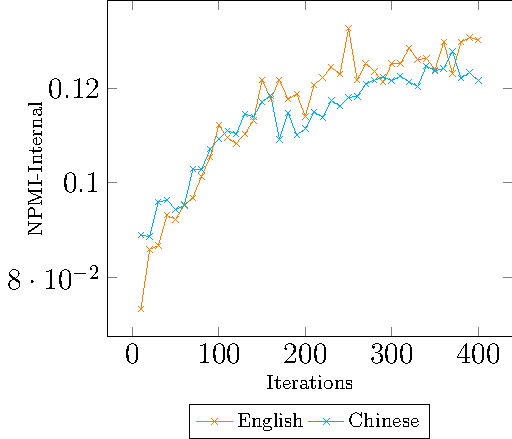
\includegraphics[height=0.5\textheight]{multilingual_itm/npmi-en-cmn.pdf}
		\end{center}
	\end{frame}
	
	\begin{frame}{English and Turkish}
		\begin{itemize}
			\item Correlation between \textbf{classification accuracy} and \textbf{NPMI-Internal}:
			\begin{itemize}
				\item English: $0.8244$
				\item Chinese: $0.6292$
			\end{itemize}
			\item Correlation between \textbf{average classification accuracy} and \textbf{NPMI-Cross}:
			\begin{itemize}
				\item $0.7963$
			\end{itemize}			
		\end{itemize}
		\begin{center}
			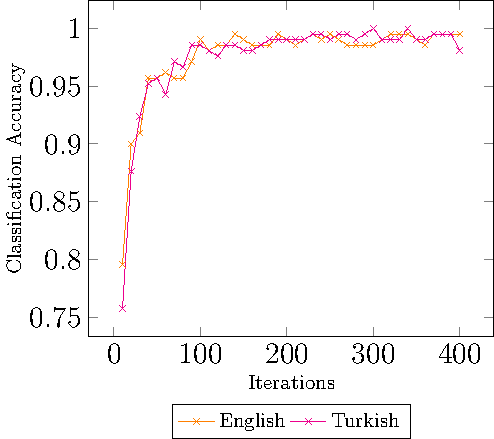
\includegraphics[height=0.5\textheight]{multilingual_itm/clf-en-tr.pdf}
			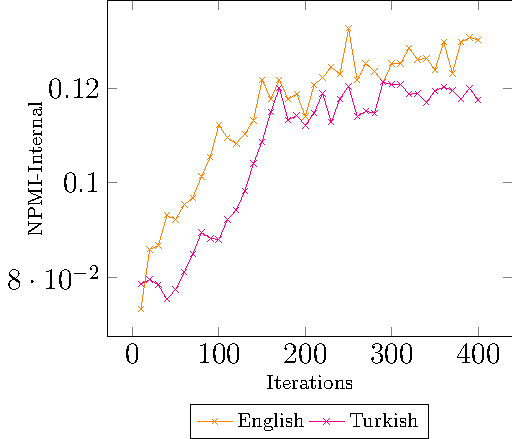
\includegraphics[height=0.5\textheight]{multilingual_itm/npmi-en-tr.pdf}
		\end{center}
	\end{frame}	


	\begin{frame}{Chinese and Turkish}
		\begin{itemize}
			\item Correlation between \textbf{classification accuracy} and \textbf{NPMI-Internal}:
				\begin{itemize}
					\item Chinese: $0.6875$
					\item Turkish: $0.6140$
				\end{itemize}
			\item Correlation between \textbf{average classification accuracy} and \textbf{NPMI-Cross}:
				\begin{itemize}
					\item $0.7394$
				\end{itemize}			
		\end{itemize}
		\begin{center}
			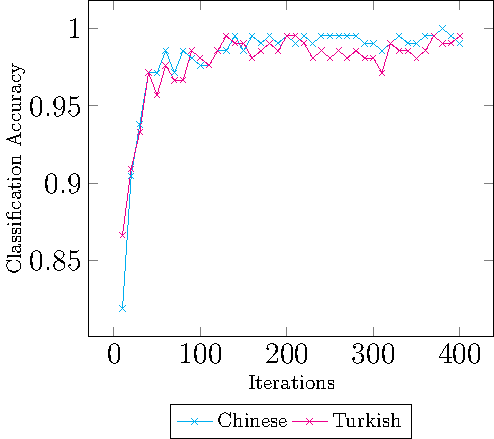
\includegraphics[height=0.5\textheight]{multilingual_itm/clf-cmn-tr.pdf}
			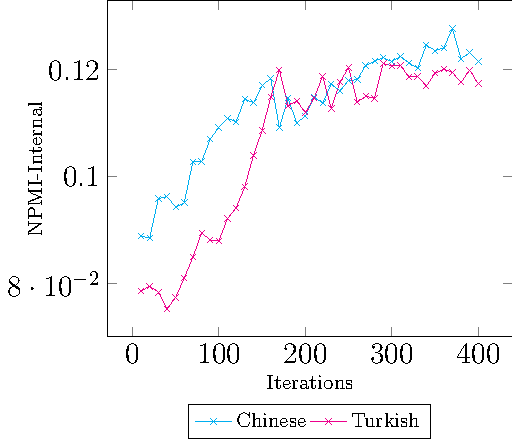
\includegraphics[height=0.5\textheight]{multilingual_itm/npmi-cmn-tr.pdf}
		\end{center}
	\end{frame}	



		\begin{frame}{Human Interpretation}
			\begin{itemize}
				\item Crowdsourcing with bilingual users
				\item Given a topic in one language
                                  and five topics in another language,
                                  see if human picks corresponding topic
				\item Experiments underway
			\end{itemize}
		\end{frame}
		\begin{frame}{Human Interpretation}
			\begin{center}
				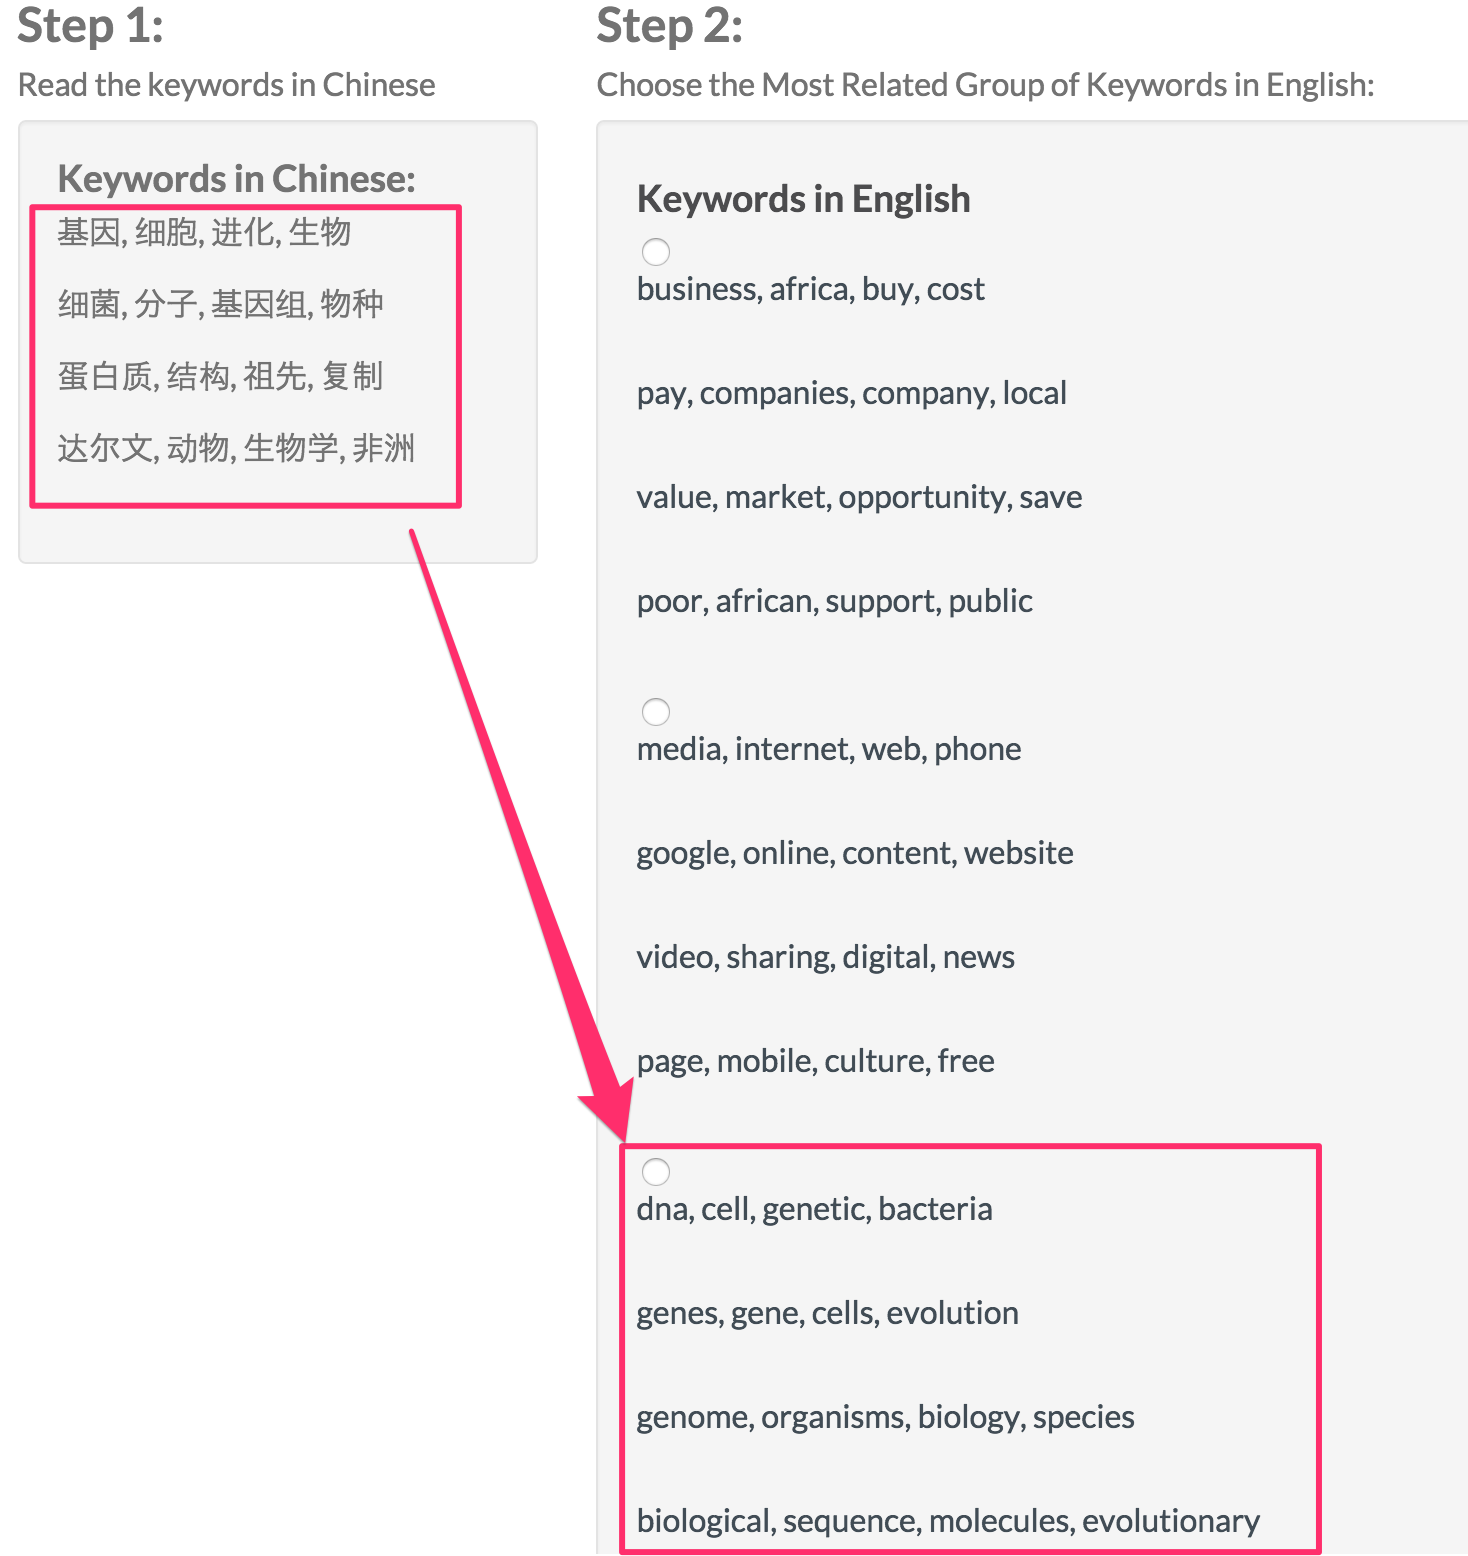
\includegraphics[height=0.8\textheight]{multilingual_itm/crowdflower.png}
			\end{center}
		\end{frame}



              \begin{frame}{Human Improvement}

                \begin{itemize}
                  \item Now that we know what a good topic looks like,
                    how can we use brief user inputs to improve model?
                    \begin{itemize}
                      \item These documents are about the same things
                        \item These words are about the same things
                          (connection to morphology / lemmatization)
                          \item Direct classification of documents (to
                            improve model)
                    \end{itemize}
                \end{itemize}

              \end{frame}


              \begin{frame}{Example on highly inflected language}

                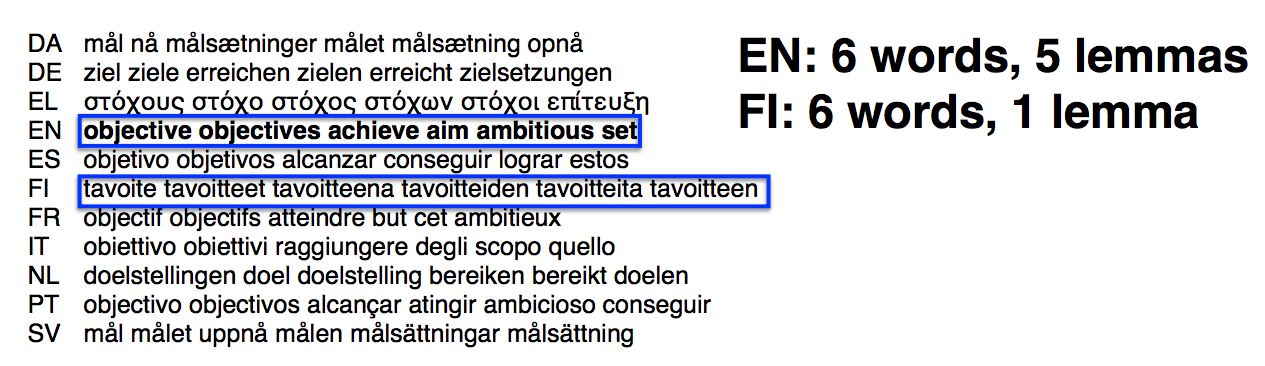
\includegraphics[width=1.0\linewidth]{multilingual_itm/morphology}

              \end{frame}

              \begin{frame}{LTDE Inputs}
                \begin{itemize}
                  \item Machine readable vector (useful for clustering
                    / visualization) of topic assignments
                  \item Human-readable topics in English and incident
                    languages
                  \item Association of documents to labels from ontology
                \end{itemize}

              \end{frame}

\end{document}
